\section{¿Que es un Outlier?}

\begin{tcolorbox}[title=Outlier]
Es un objeto que tiene características diferentes de la mayoria de otros
del dataset con el que estemos trabajando. También puede ser un valor
inusual con respecto a los valores típicos de una variable.
\end{tcolorbox}

Por ejemplo, si tenemos un dataset con la información de la altura de un
grupo de personas, y el promedio es de 1.80 metros, un outlier sería ver
un valor de 2.15 metros.

La naturaleza de los outliers es dual, así como pueden ser el resultado
de errores de medición o entrada de datos, también pueden representar
eventos geniunos pero poco frencuentes que aún nos pueden dar
información valiosa del conjunto de datos. \cite{Munoz_outliers}

\begin{figure}[H]
\centering 
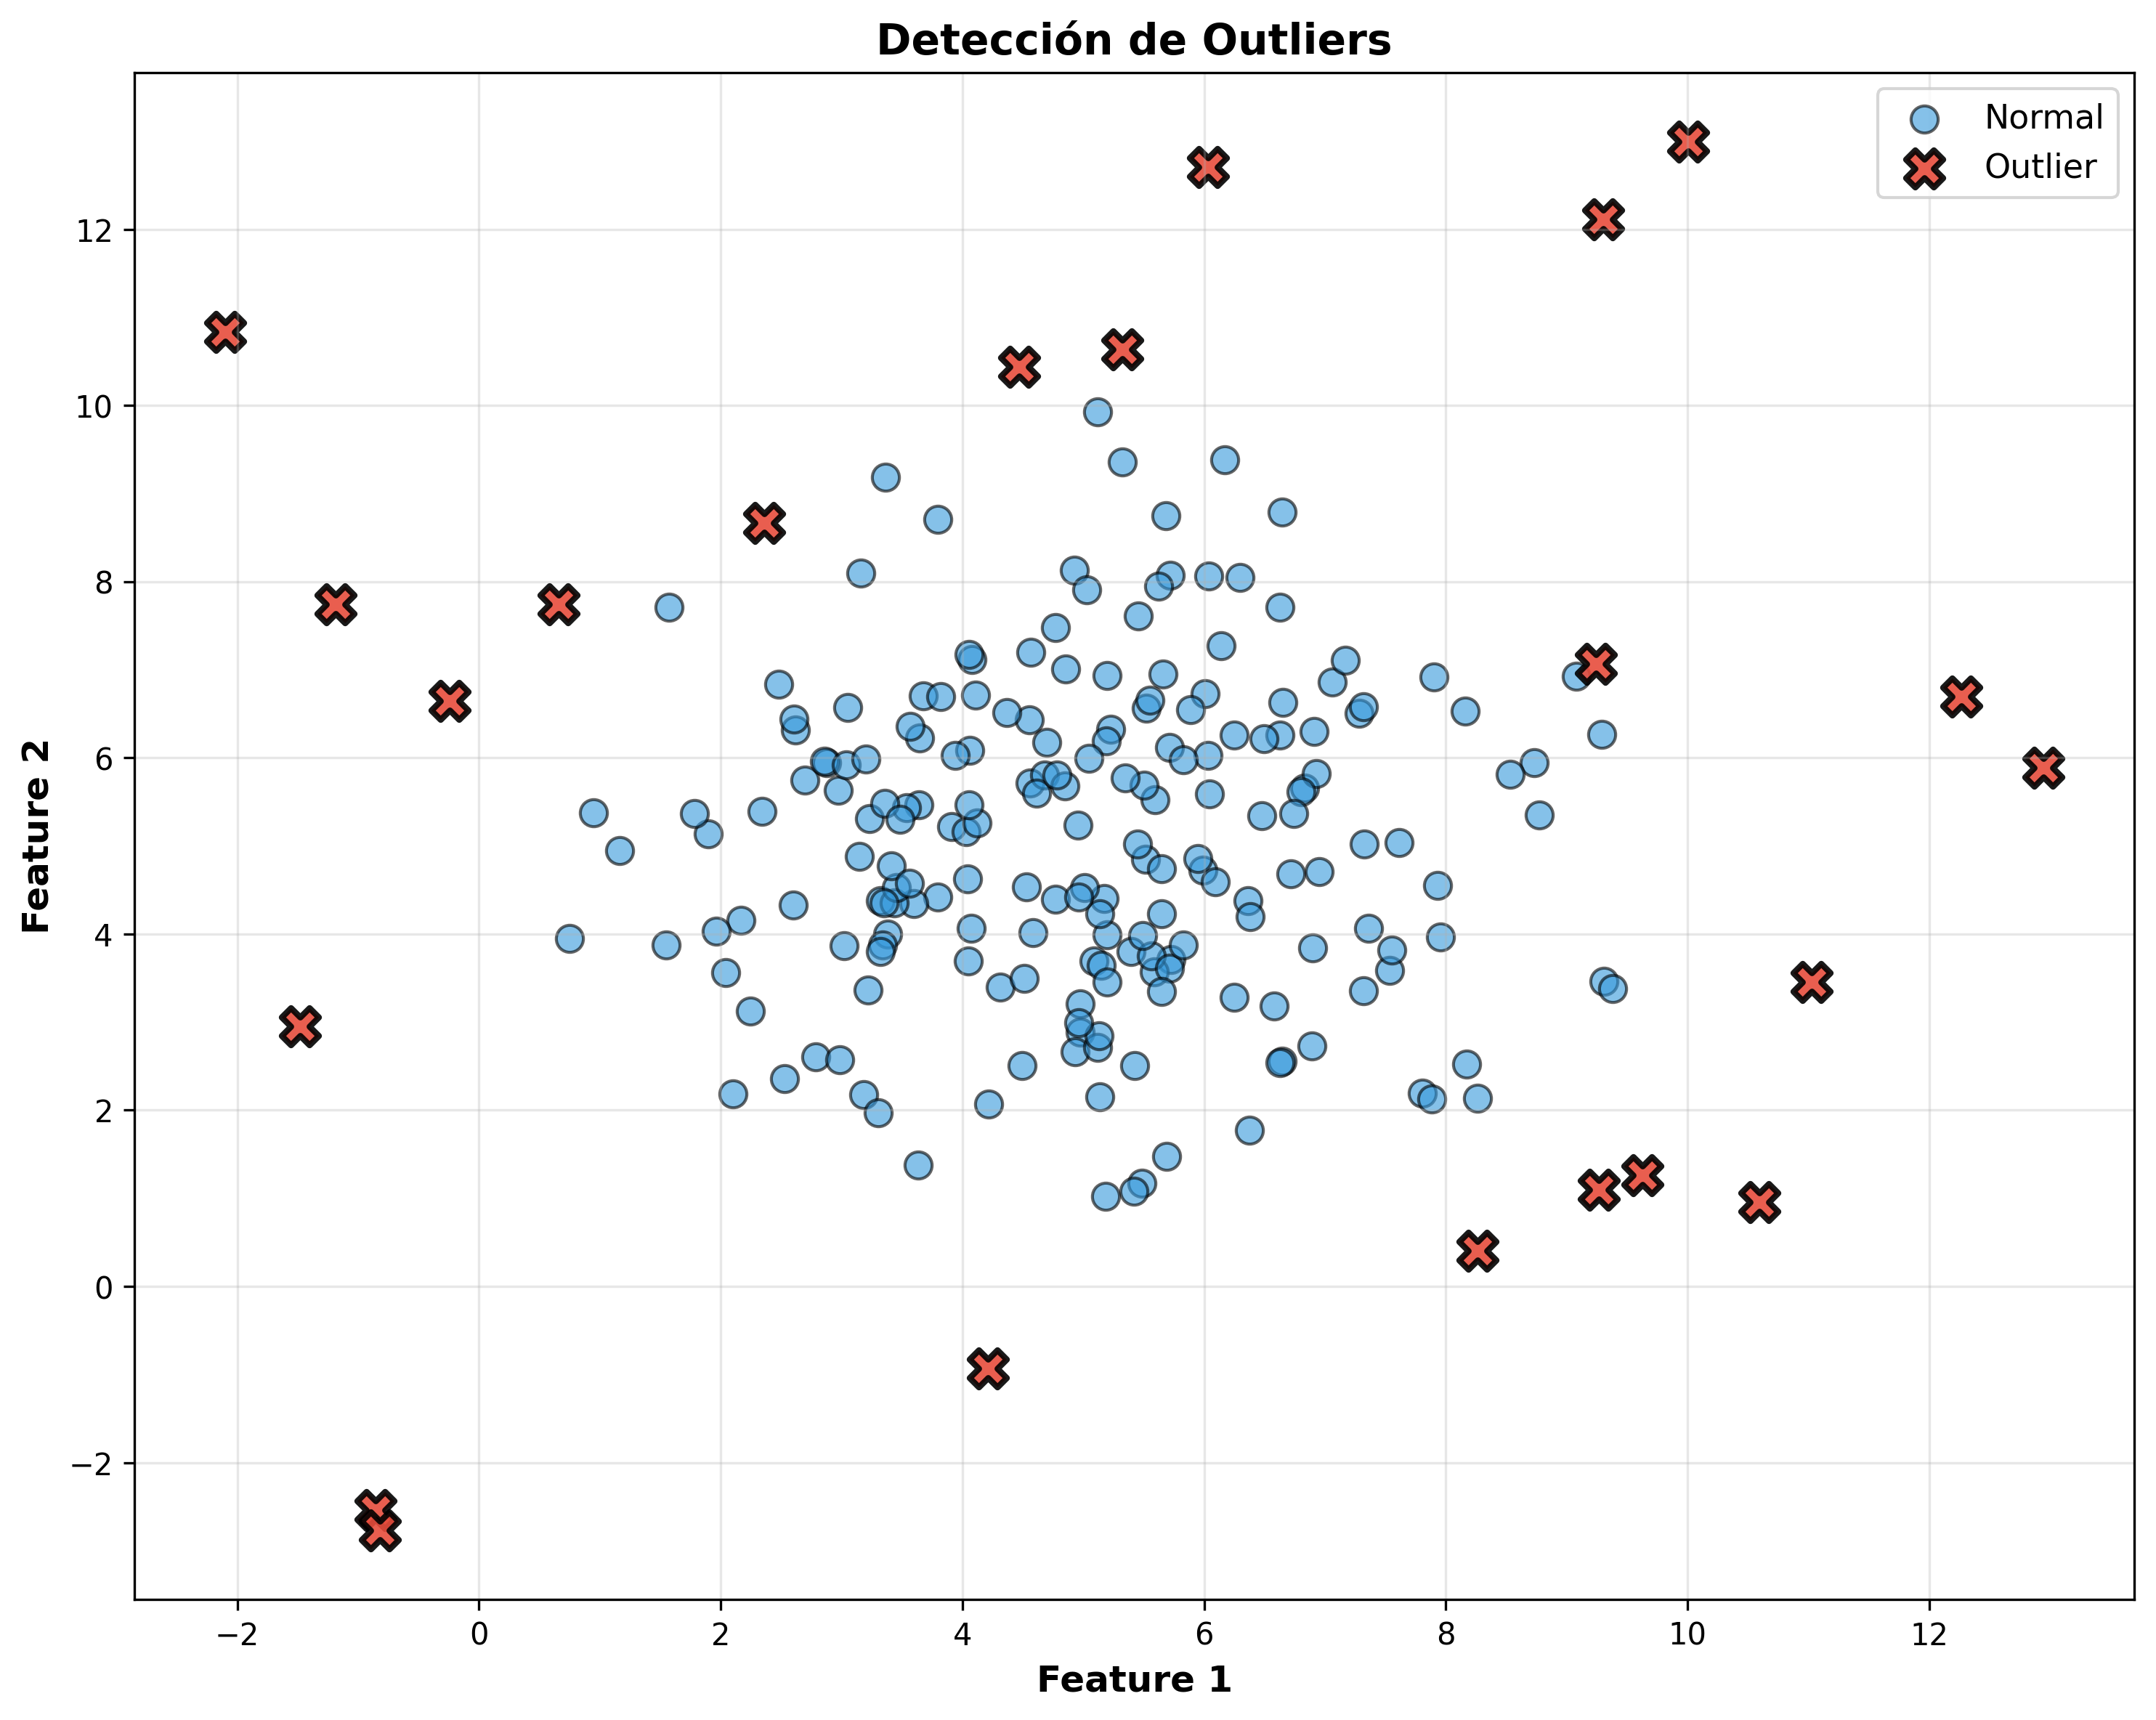
\includegraphics[scale=0.6]{imagenes/outliers.png}
\caption{Visualización de outliers}
\end{figure}

\subsection{La Z-score y el IQR para detectar outliers}

Los outliers se detectan mediante su 'Z-score', que es una medida de
cuántas desviaciones estándar un dato se encuentra por encima o por
debajo de la media del conjunto de datos. Un valor de Z-score mayor a 3
o menor a -3 generalmente se considera un outlier, aunque este umbral
puede ajustarse según el contexto y la naturaleza de los datos. Esta
calificación se calcula usando la fórmula:

\[Z = \frac{X - \mu}{\sigma}\]

Donde:

\begin{itemize}
\item
  \(X\) es el valor del dato que se está evaluando,
\item
  \(\mu\) es la media del conjunto de datos,
\item
  \(\sigma\) es la desviación estándar del conjunto de datos.
\end{itemize}

Otra forma de describirlo es mediante el rango intercuartílico (IQR),
que se calcula como la diferencia entre el tercer cuartil (Q3) y el
primer cuartil (Q1) de los datos. Un dato se considera un outlier si
está por debajo de \(Q1 - 1.5 \times IQR\) o por encima de
\(Q3 + 1.5 \times IQR\).

Calcularlo es más trivial que el Z-score, pero es menos preciso, ya que
no toma en cuenta la distribución de los datos, sino solo su posición
relativa a los cuartiles. Se calcula como:

\[IQR = Q3 - Q1\]

Donde:

\begin{itemize}
\item
  \(Q1\) es el primer cuartil (25\% de los datos por debajo de este
  valor),
\item
  \(Q3\) es el tercer cuartil (75\% de los datos por debajo de este
  valor).
\end{itemize}

\subsection{¿Por qué es importante detectar los outliers?}

Si estos valores no se identifican ni procesan de una manera adecuada
perjudica considerablemente los análisis estadísticos que se hagan de
nuestros datos, ya que puede sesgar el modelos, reducir su precisión y/o
comprometer su interpretabilidad.

Sin embargo la decisión de cómo manejar un outlier debe precederse por
una investigación sobre \emph{por qué existe}. Si un outlier es
claramente el resultado de un error su eliminación o corrección es
justificada. Sin embargo, si el outlier representa un evento genuino y
válido, pero tal vez menos probable, debe ser considerado cuidadosamente
o incluso aprovechado para obtener información valiosa. \cite{Pontia_2026}

\subsection{Outliers y Ruido}

Algo que vale la pena recalcar es que un outlier \textbf{no es lo mismo}
que el ruido. Mientras que el ruido son datos incorrectos o
inconsistentes que restan la calidad del modelo que se vaya a crear, un
outlier es más un valor que es posible pero muy poco frecuente.

\section{Categorización de Outliers}\

\subsection{Outliers Globales}

Son los outliers menos específicos. Son eventos que se desvían
significativamente del resto del dataset. Por ejemplo, un conjunto de
datos de edad de personas en una empresa y un dato anómalo de 150 años.

\subsection{Outliers Contextuales}

Estos eventos se consideran atípicos según el contexto específico bajo
el que se vayan a tratar. Por ejemplo, si nuestro dataset es sobre
temperaturas en un estado a lo largo del año, un valor de 30°C es normal
en verano, pero atípico en invierno.

\subsection{Outliers Colectivos}

Como su nombre lo dice, son eventos que aunque de manera individual no
parecen ser anómalos, en conjunto si representan una anomalía. Por
ejemplo, el rechazo de envío de un paquete de una computadora a otra se
considera normal, pero si varias computadoras continúan enviando
paquetes rechazados unas a otras, el conjunto se debería considerar como
outlier colectivo. \cite{MineriaDatos_R}

\begin{figure}[H]
\centering
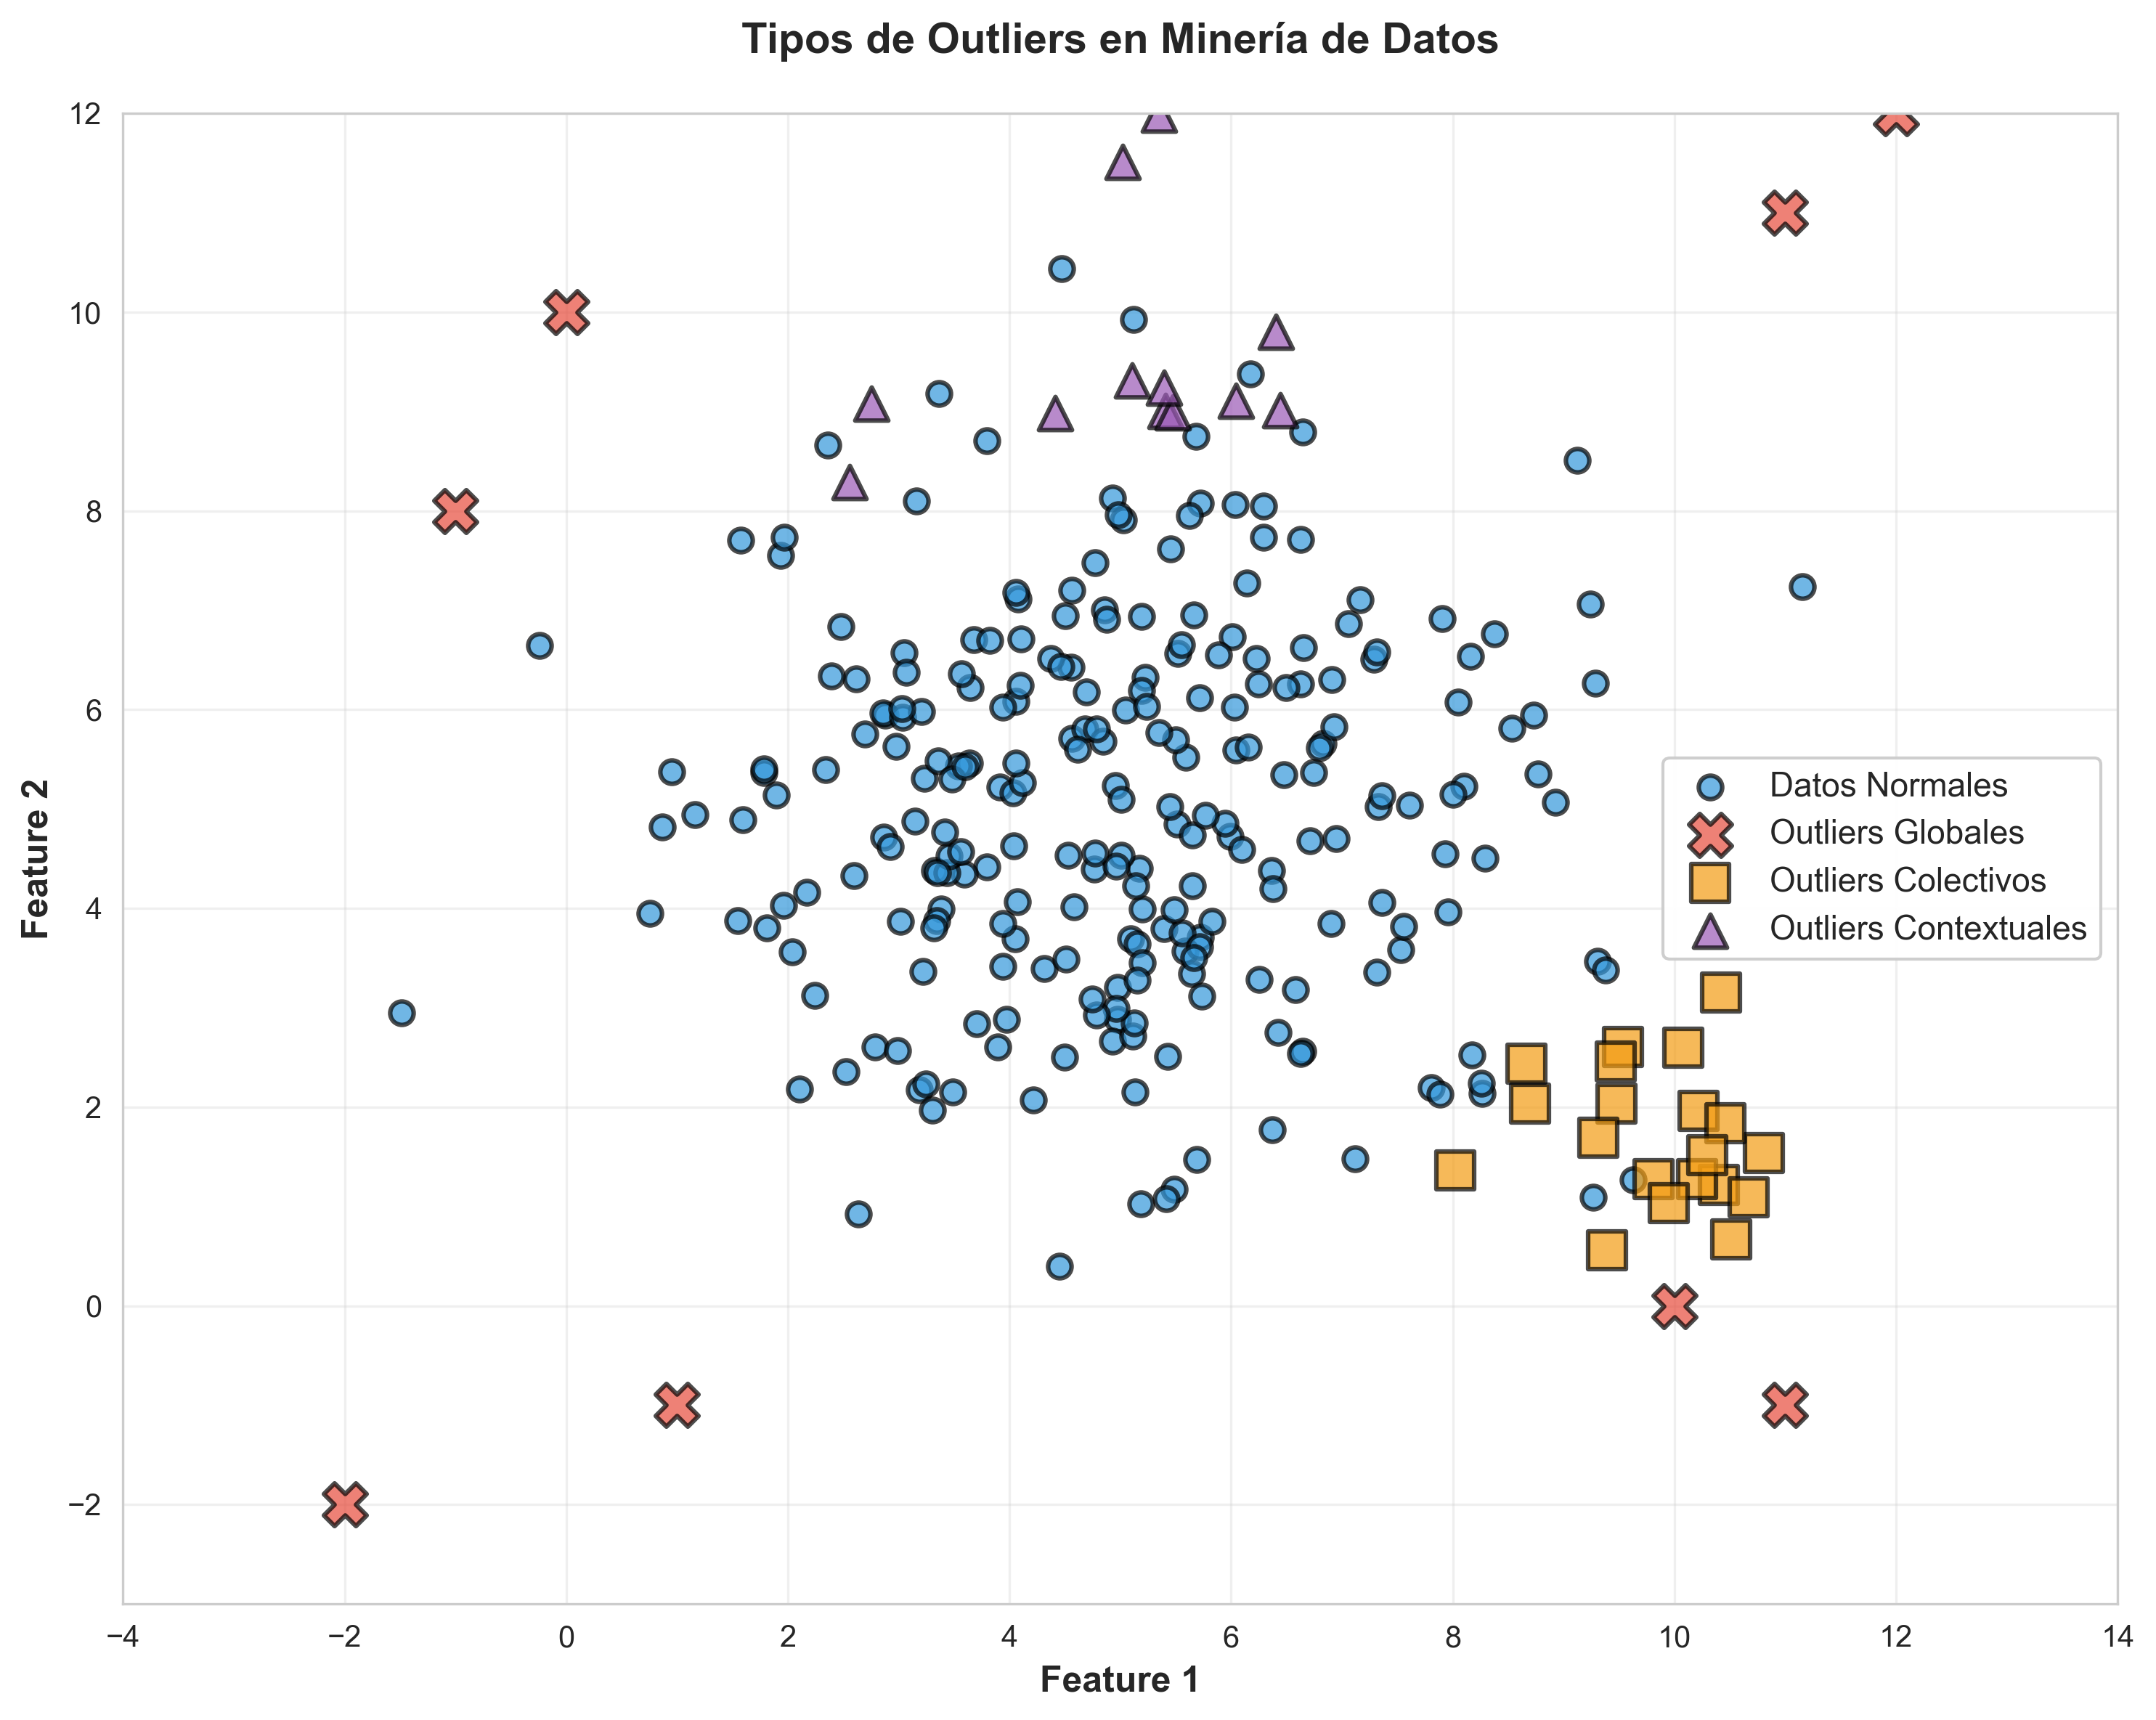
\includegraphics[scale=0.6]{imagenes/tipos_outliers.png}
\caption{Visualización de tipos de Outliers}
\end{figure}

\section{Clustering}

\begin{tcolorbox}[title=Clustering]
El clustering es una técnica de aprendizaje automático no supervisado
que busca dividir el dataset en el que se este trabajando en grupos, a
los que llamaremos \emph{\emph{clústers}}, en donde los elementos que se
encuentran dentro de uno son lo más similares entre si y lo más
distintos posibles o los de otro clúster.
\end{tcolorbox}

Como es un método no supervizado no se necesita que los datos tengan
etiquetas, clasificaciones previas o ejemplos de entrenamiento, si no
que más bien lo que se busca es encontrar la distancia matemática (o
similitud) entre cada dato para agruparlos lo más correctamente posible.

\subsection{¿De qué nos sirven los clústers?}

\begin{itemize}
\item
  \textbf{Descubrir patrones ocultos}: Ayuda a revelar relaciones,
  estructuras y agrupaciones naturales dentro de los datos que no son
  evidentes a simple vista.
\item
  \textbf{Simplificar información compleja}: Permite dividir y resumir
  grandes volúmenes de datos ruidosos en subgrupos más pequeños,
  homogéneos y manejables.
\item
  \textbf{Exploración y descubrimiento}: Es sumamente útil para
  encontrar grupos de datos o categorías que eran previamente
  desconocidas por los analistas.
\end{itemize}

\section{Algoritmos de Clustering}

\subsection{Términos Generales de los Algoritmos de Clústering}

\begin{enumerate}
\item
  El algoritmo evalúa cada registro del conjunto de datos tomando en
  cuenta sus características como si fueran coordenadas de un punto en
  el espacio.
\item
  Luego, usamos métricas (como la distancia euclídea o la correlación)
  para medir qué tan cerca están esos puntos unos de otros
\item
  Con base en esta proximidad, el algoritmo asocia los puntos de modo
  que se minimice la distancia entre los elementos de un mismo grupo
  (haciéndolos muy compactos y similares) y se maximice la separación
  con los demás grupos.
\end{enumerate}

\subsubsection{Ejemplo Corto de Clustering}

Digamos que tenemos un dataset de compras de un supermercado. Cada
entrada en el conjunto se refiere a lo que compra una persona y queremos
detectar grupos basados en clustering en base a esos datos. Entonces el
algoritmo puede agrupar en 'compradores frecuentes', 'compradores
nuevos', 'compradores de un solo artículo', etc. Y en base a estas
métricas el supermercado puede encontrar patrones de los artículos más
vendidos, etc.

\subsection{La Distancia Euclídea}

Como mencionabamos, una de las métricas más comunes para medir la
similitud entre puntos es la distancia euclídea. Esta se calcula usando
la fórmula:

\[d(P, Q) = \sqrt{\sum_{i=1}^{n} (p_i - q_i)^2}\]

Donde: - \(P\) y \(Q\) son dos puntos en un espacio n-dimensional,
representados por sus coordenadas \(p_i\) y \(q_i\) respectivamente. -
\(n\) es el número de dimensiones o características que describen cada
punto.

La distancia euclídea mide la longitud del segmento de línea recta entre
los puntos \(P\) y \(Q\) en el espacio n-dimensional. Cuanto menor sea
esta distancia, más similares son los puntos entre sí.

\section{K-Means}

El algoritmo de K-Means es uno de los métodos de clustering más
populares y ampliamente utilizados. Su objetivo es dividir un conjunto
de datos en \(k\) clústers distintos, donde \(k\) es un número
predefinido por el usuario, minimizando la suma euclídea de las
distancias al cuadrado entre los puntos. Funciona de la siguiente
manera:

\begin{itemize}
\item
  Tomamos \(k\) datos (o puntos) aleatorios como los centros iniciales
  (o \emph{centroides}) de cada clúster.
\item
  Asignamos el resto de los datos a el clúster más cercano calculando su
  distancia euclídea a cada centro y asignandolo al de menor distancia.
\item
  Una vez que todos los datos han sido asignados a un clúster, el
  algoritmo recalcula los centros de cada clúster tomando la media de
  los puntos asignados a ese clúster.
\item
  Repetimos los pasos de asignación y recalculo de centros hasta que las
  asignaciones de los puntos no cambien significativamente o se alcance
  un número máximo de iteraciones.
\end{itemize}

\subsection{Los Centroides}

Mencionamos antes que éstos son los puntos que representan el centro de
cada clúster. Se calculan tomando la media de las coordenadas de los
puntos asignados a cada clúster, siendo así la 'coordenada promedio'
de los puntos dentro del clúster. Matemáticamente, se ve de la siguiente
manera:

\[\mu_i = \frac{1}{|S_i|} \sum_{x \in S_i} x\]

Donde:

\begin{itemize}
\item
  \(\mu_i\) es el centroide del clúster \(i\),
\item
  \(S_i\) es el conjunto de puntos asignados al clúster \(i\)
\item
  \(|S_i|\) es el número de puntos en el clúster \(i\),
\item
  \(x\) representa cada punto dentro del clúster \(i\).
\end{itemize}

\subsection{La Inercia de K-Means}

Otro objetivo de K-Means es minimizar la suma de las distancias al
cuadrado entre cada punto y el centroide de su clúster asignado, esto
para saber que tan dispersos están los datos respecto a su centroide.
Matemáticamente, esto se expresa como

\[\sum_{j=1}^{k} \sum_{x \in S_j} d(x, \mu_j)^2\]

Donde:

\begin{itemize}
\item
  \(S_j\) es el conjunto de puntos asignados al clúster \(j\),
\item
  \(\mu_j\) es el centroide del clúster \(j\),
\item
  \(d(x, \mu_j)\) es la distancia entre el punto \(x\) y el centroide
  \(\mu_j\).
\end{itemize}

\subsection{Visualizando K-Means}

Por ejemplo, en las siguientes imágenes tenemos un dataset con una \(n\)
cantidad de datos. Vamos a tomar \(k=3\) y seleccionamos 3 puntos
aleatorios y los marcamos con azul, verde y amarillo. De esto creamos
los primeros clústeres basándonos en la distancia de cada punto al
centroide. Luego, recalculamos los centroides tomando la media de los
puntos asignados a cada clúster y repetimos el proceso hasta que los
clústeres no cambien significativamente. \cite{Google_kMeans}

\begin{figure}[H]
\centering
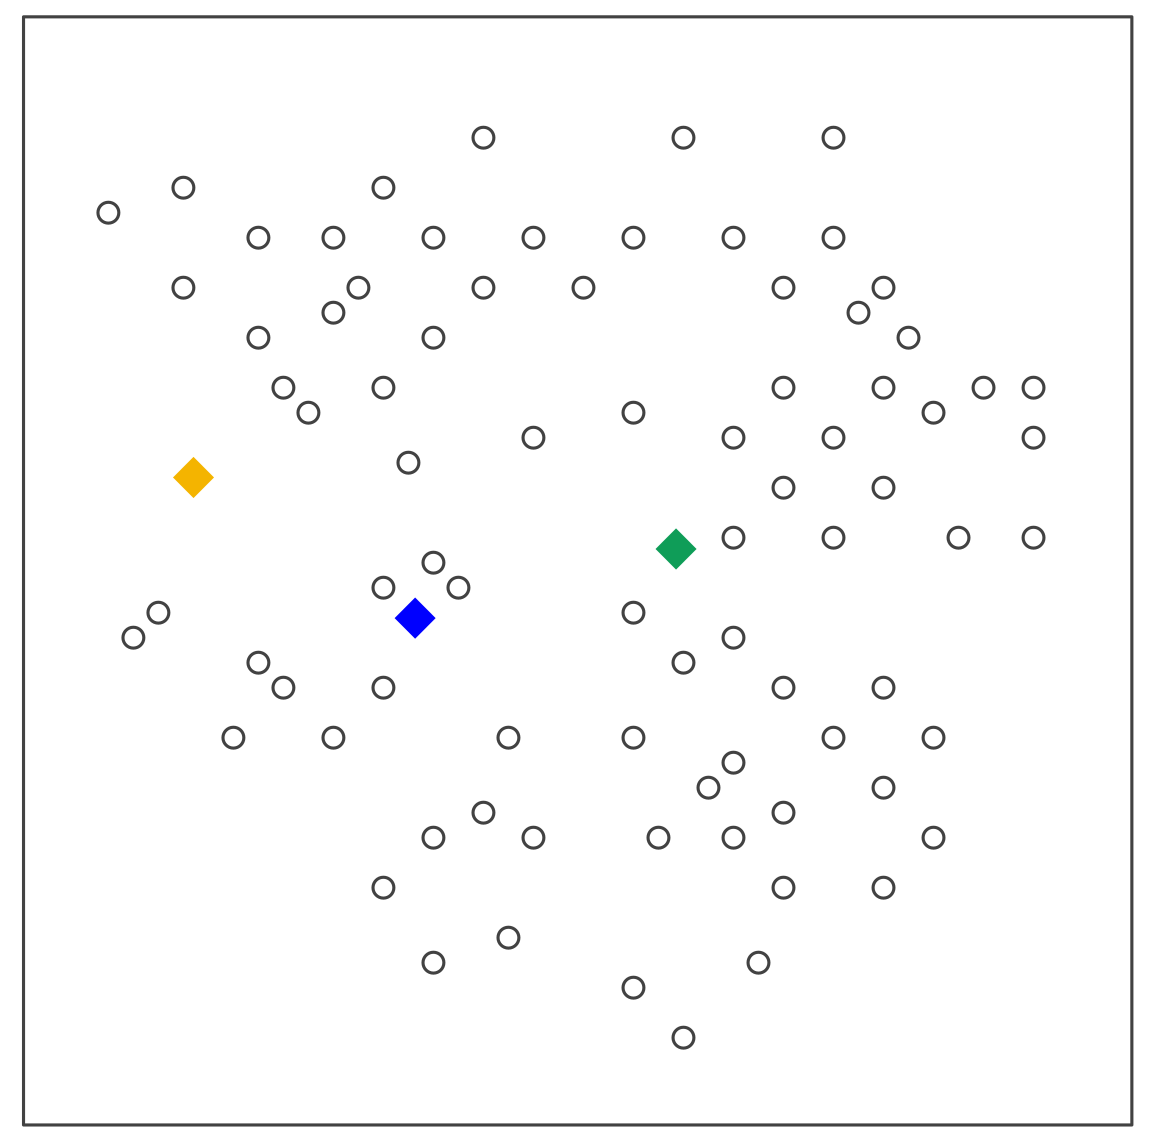
\includegraphics[scale=0.7]{imagenes/paso1_kmeans.png}
\caption{Inicialización de K-Means con $k=3$}
\end{figure}

\begin{figure}[H]
\centering
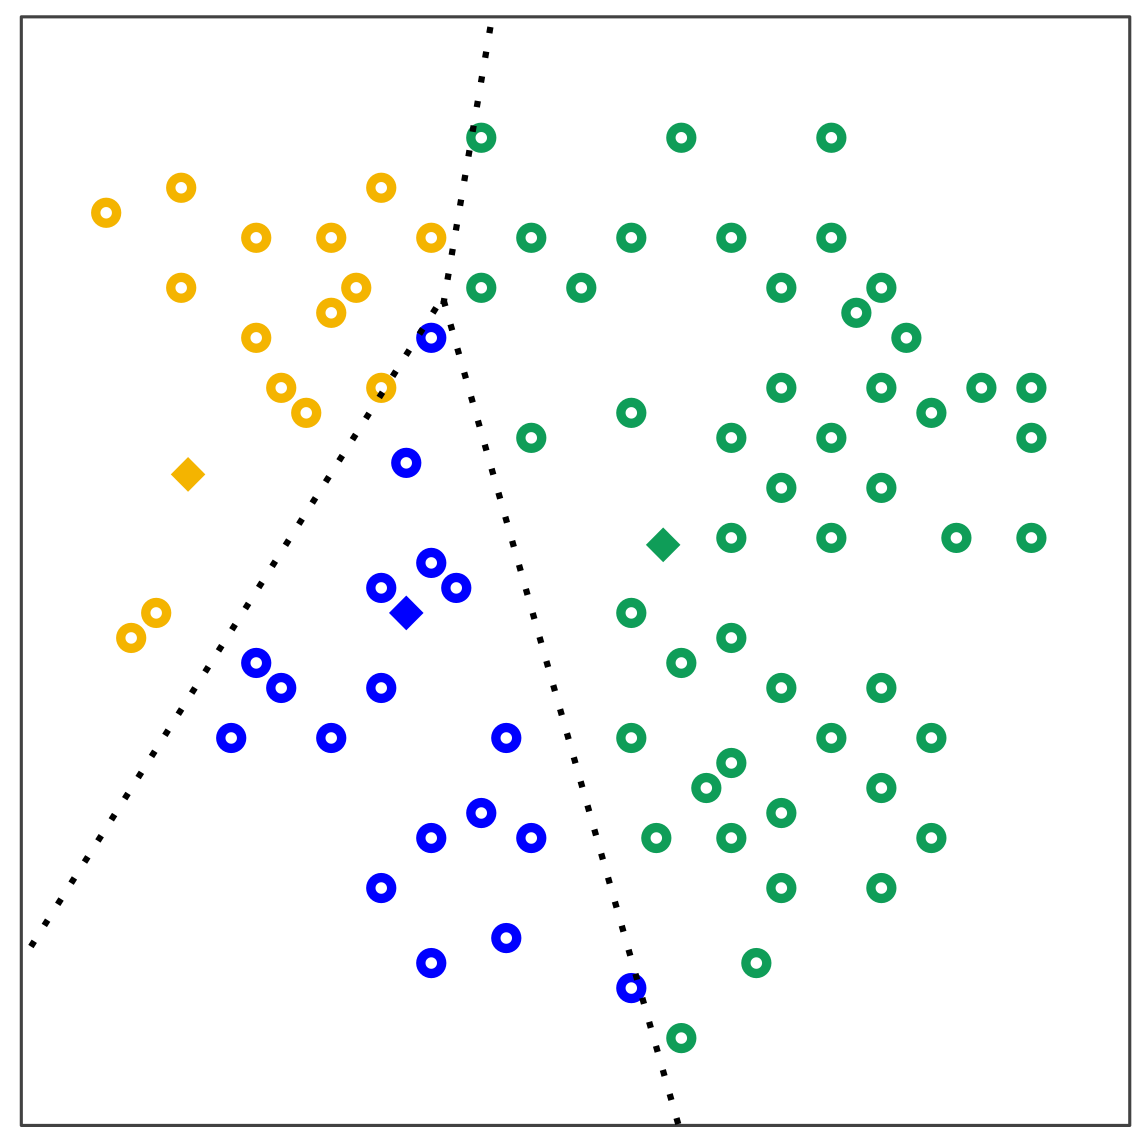
\includegraphics[scale=0.7]{imagenes/paso2_kmeans.png}
\caption{Clústeres Iniciales}
\end{figure}

\begin{figure}[H]
\centering
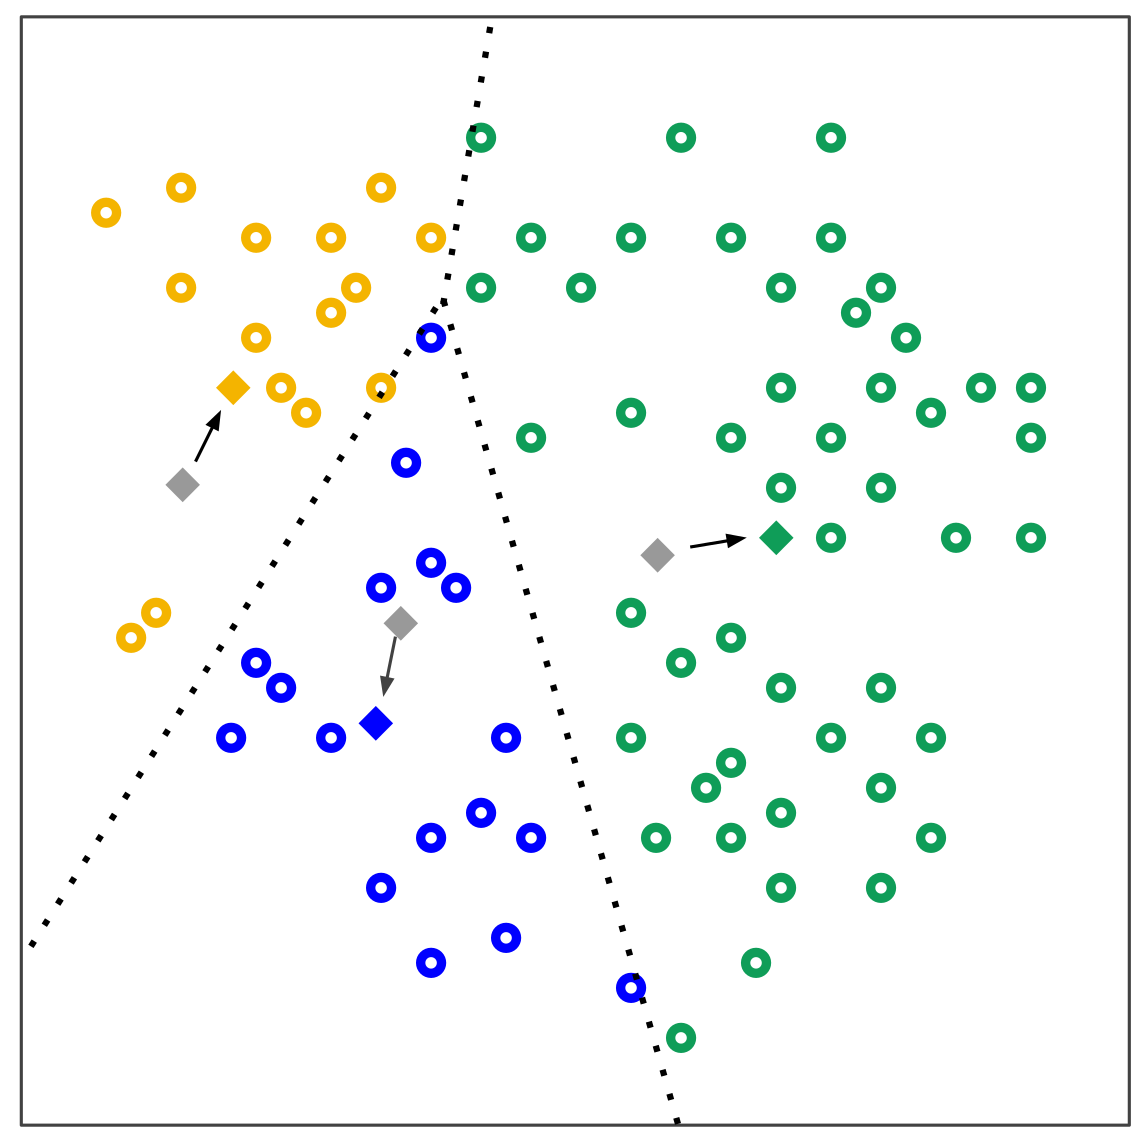
\includegraphics[scale=0.7]{imagenes/paso3_kmeans.png}
\caption{Centroides recalculados}
\end{figure}

\begin{figure}[H]
\centering
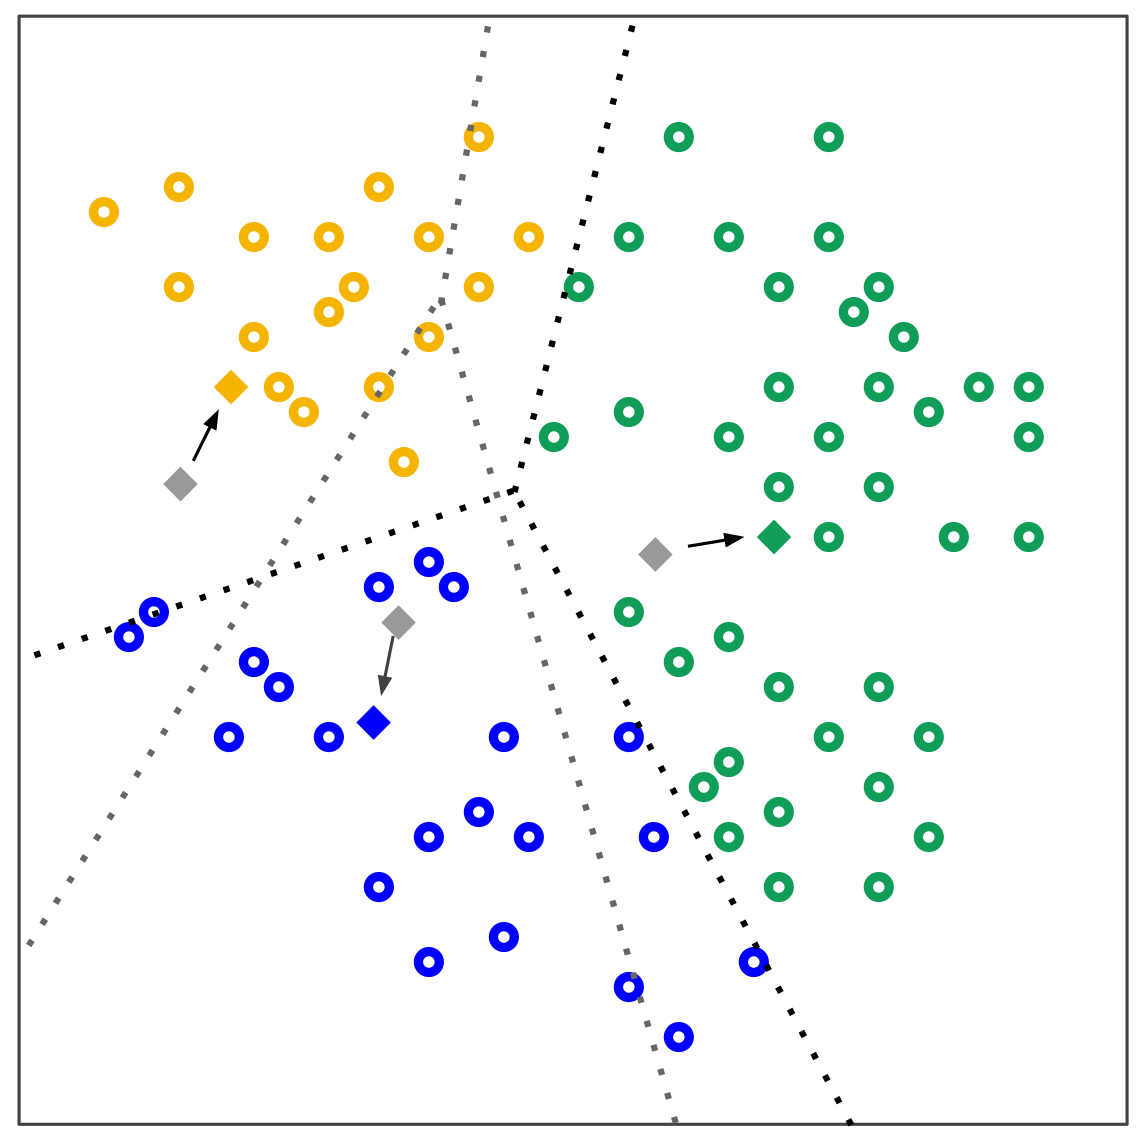
\includegraphics[scale=0.7]{imagenes/paso4_kmeans.png}
\caption{Clústeres Finales}
\end{figure}

\subsection{Ejemplo de Uso: El consumo eléctico en hogares}

Para ilustrar el funcionamiento de k-means en la detección de datos
atípicos, analizaremos un dataset real de consumo eléctrico doméstico,
proveniente del
\href{https://archive.ics.uci.edu/dataset/235/individual+household+electric+power+consumption}{repositorio
UCI}. Este dataset contiene mediciones minuto a minuto de la potencia
activa consumida y el voltaje registrado en una vivienda francesa desde
Diciembre de 2006 hasta Noviembre de 2010.

Al aplicar k-means a este dataset, podemos identificar patrones de
consumo y detectar posibles outliers que podrían indicar anomalías en el
consumo eléctrico, como picos inusuales o caídas repentinas.

\begin{enumerate}
\item
  \textbf{Selección y limpieza de variables:} Se utilizan dos variables
  principales:

  \begin{itemize}
  \item
    \texttt{Global\_active\_power} (potencia activa global, en kW)
  \item
    \texttt{Voltage} (voltaje de la red, en V) Se eliminan valores nulos
    y se convierten los datos a formato numérico.
  \end{itemize}
  
\item
  \textbf{Escalamiento:} Dado que ambas variables tienen escalas muy
  distintas, se normalizan para evitar que una domine el análisis de
  distancias. Usaremos \texttt{StandardScaler} de
  \texttt{sklearn.preprocessing} para centrar los datos en torno a la
  media y escalar a la unidad de varianza.

  \begin{tcolorbox}[title=Nota sobre StandardScaler]
  Nota: \texttt{StandardScaler} usa la fórmula
  $x_{scaled} = \frac{x - \bar{x}}{s}$ para normalizar los datos, donde
  \(\bar{x}\) es la media de la variable y \(s\) es su desviación
  estándar. Esto asegura que cada variable tenga una media de 0 y una
  desviación estándar de 1, lo que facilita la comparación entre ellas en
  el análisis de clustering.
  \end{tcolorbox}


\item
  \textbf{Aplicación de k-means:} Se agrupan los datos en $k$
  clústeres (supondremos \(k=8\)). Para cada registro, se calcula la
  distancia al centroide de su grupo. Usaremos el algoritmo de k-means
  de \texttt{sklearn.cluster} para realizar esta tarea.
  
\item
  \textbf{Identificación de atípicos:} Los registros cuya distancia al
  centroide supera un percentil alto (por ejemplo, el 99\%) se marcan
  como atípicos.

  \begin{itemize}
  \item
    \textbf{Atípicos globales:} Potencias inusualmente altas, sin
    importar el voltaje.
  \item
    \textbf{Atípicos contextuales:} Consumos normales pero asociados a
    voltajes anómalos.
  \end{itemize}
  
\item
  \textbf{Visualización:} Se genera un gráfico interactivo donde los
  puntos atípicos se resaltan en rojo, permitiendo explorar visualmente
  la estructura y los extremos del dataset.
\end{enumerate}

\begin{tcolorbox}[title=Nota sobre los resultados]
Los resultados mostrados a continuación son fijos debido a la naturaleza
de LaTeX, pero se puede consultar
\href{https://molab.marimo.io/notebooks/nb_SjX8JxW8MgH6GjkQaARuKq}{este
cuaderno de Marimo} para ver un análisis interactivo al modificar la
cantidad de clústers y el umbral de detección de atípicos.
\end{tcolorbox}


\begin{lstlisting}[language=Python, caption=Ejecución de K-Means para detección de outliers en consumo eléctrico]
import pandas as pd
import numpy as np
import matplotlib.pyplot as plt
from sklearn.cluster import KMeans
from sklearn.datasets import make_blobs
import plotly.express as px
from sklearn.preprocessing import StandardScaler

# Cargamos el dataset y seleccionamos/limpiamos las variables de interes
df = pd.read_csv('datasets/household_power_consumption.txt', sep=';', nrows= 10000, low_memory=False)
df_limpio = df[['Global_active_power', 'Voltage']].replace('?', np.nan).dropna().astype(float)
scaler = StandardScaler()
df_scaled = scaler.fit_transform(df_limpio)

# Aplicamos k-means para agrupar los datos en clusters y detectar atipicos
# Como mencionabamos, vamos a suponer $k=8$. Pero como saber si este es el valor
# correcto?
kmeans = KMeans(n_clusters=8, random_state=42)
df_limpio['Cluster'] = kmeans.fit_predict(df_scaled)

# Obtenemos las coordenadas de los centroides y calculamos la distancia de cada 
# punto a su centroide correspondiente
centroides = kmeans.cluster_centers_
distancias = np.sqrt(np.sum((df_scaled - centroides[df_limpio['Cluster']]) ** 2, axis=1))

# El porcentaje de los datos mas lejanos a cualquier cluster se consideran atipicos
umbral = np.percentile(distancias, 99)  # Ajustable segun el nivel de sensibilidad deseado
df_limpio['Es_Atipico'] = distancias > umbral

# Creamos una columna de texto para formatear las leyendas de forma clara
df_grafico = df_limpio.copy()
df_grafico['Clasificacion'] = df_grafico['Cluster'].astype(str)
df_grafico.loc[df_grafico['Es_Atipico'], 'Clasificacion'] = 'Atipico'

# Mapa de colores: clusteres comunes y rojo para anomalias
mapa_colores = {
    '0': '#1f77b4',      # Azul
    '1': '#2ca02c',      # Verde
    '2': '#9467bd',      # Morado
    '3': '#bcbd22',      # Amarillo
    '4': '#17becf',      # Cian
    '5': '#e377c2',      # Rosa
    '6': '#ff7f0e',      # Naranja
    '7': '#8c564b',      # Cafe
    '8': '#7f7f7f',      # Gris
    '9': '#ffbb78',      # Naranja claro
    'Atipico': '#d62728' # Rojo para Outliers
}

# Construccion del scatter plot interactivo
fig = px.scatter(
    df_grafico,
    x='Global_active_power',
    y='Voltage',
    color='Clasificacion',
    color_discrete_map=mapa_colores,
    symbol='Clasificacion',
    opacity=0.6,
    title='Deteccion de Atipicos (K-Medias)',
    labels={
        'Global_active_power': 'Potencia Activa Global (kW)',
        'Voltage': 'Voltaje (V)'
    },
    # Muestra datos limpios al pasar el cursor
    hover_data={'Cluster': True, 'Es_Atipico': False} 
)

fig.update_layout(
    legend_title_text='Estructura del Dataset',
    margin=dict(l=40, r=40, t=60, b=40)
)
\end{lstlisting}

\begin{figure}[H]
\centering
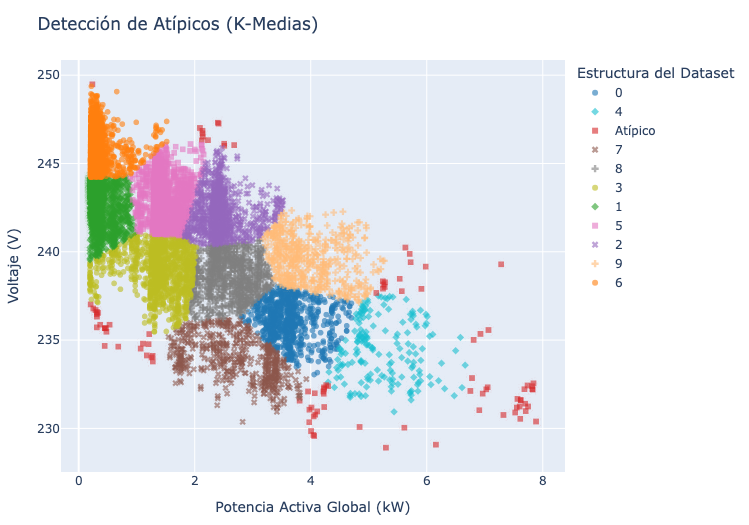
\includegraphics[scale=0.7]{imagenes/plot_consumo_electrico.png}
\caption{Visualización de K-Means con detección de atípicos en consumo eléctrico}
\end{figure}


\subsection{La Regla del Codo}

¿Y cómo sabemos cual es el valor correcto de \(k\) a considerar? El
método del codo sirve justo para esto. Funciona de la siguiente manera:

\begin{itemize}
\item
  Ejecutamos \(k\)-Means para diferentes valores de \(k\) (por ejemplo,
  desde 1 hasta 10).
\item
  Para cada valor de \(k\), calculamos la inercia.
\item
  Luego, graficamos la inercia en función de \(k\) y buscamos el punto
  donde la disminución de la inercia comienza a ser menos pronunciada,
  formando una especie de codo (de ahi el nombre).
\item
  El punto resultante suele ser la mejor elección para el número óptimo
  de clústers, ya que representa un buen equilibrio entre la complejidad
  del modelo (número de clústers) y la calidad del ajuste (inercia).
\end{itemize}

\subsubsection{Ejemplo usando el método del codo}

Veamos como se ve esto aplicado a nuestro dataset anterior. En este caso, vamos a ejecutar k-means 
para valores de $k$ desde 1 hasta 10 y graficar la inercia para cada uno de estos valores.

\begin{lstlisting}[language=Python, caption=Ejemplo del método del codo para determinar el número óptimo de clústers]
def elbow_method(data, max_clusters=10):
    """
    Aplica el metodo del codo para seleccionar el numero optimo de clusters en k-means.

    Parametros:
    ----------
    data : matriz o matriz dispersa, forma (n_samples, n_features)
        Los datos de entrada.

    max_clusters : int, opcional (por defecto=10)
        El numero maximo de clusters a considerar.
    """

    sum_of_squared_distances = []

    for k in range(1, max_clusters+1):
        kmeans = KMeans(n_clusters=k)
        kmeans.fit(data)
        sum_of_squared_distances.append(kmeans.inertia_)

    # Graficar la curva del codo
    plt.plot(range(1, max_clusters+1), sum_of_squared_distances, 'bx-')
    plt.xlabel('Numero de Clusters (k)')
    plt.ylabel('Suma de las Distancias al Cuadrado')
    plt.title('Curva del Codo')
    plt.show

# Aplicar el metodo del codo
elbow_method(df_limpio, max_clusters=10)
\end{lstlisting}

\begin{figure}[H]
\centering
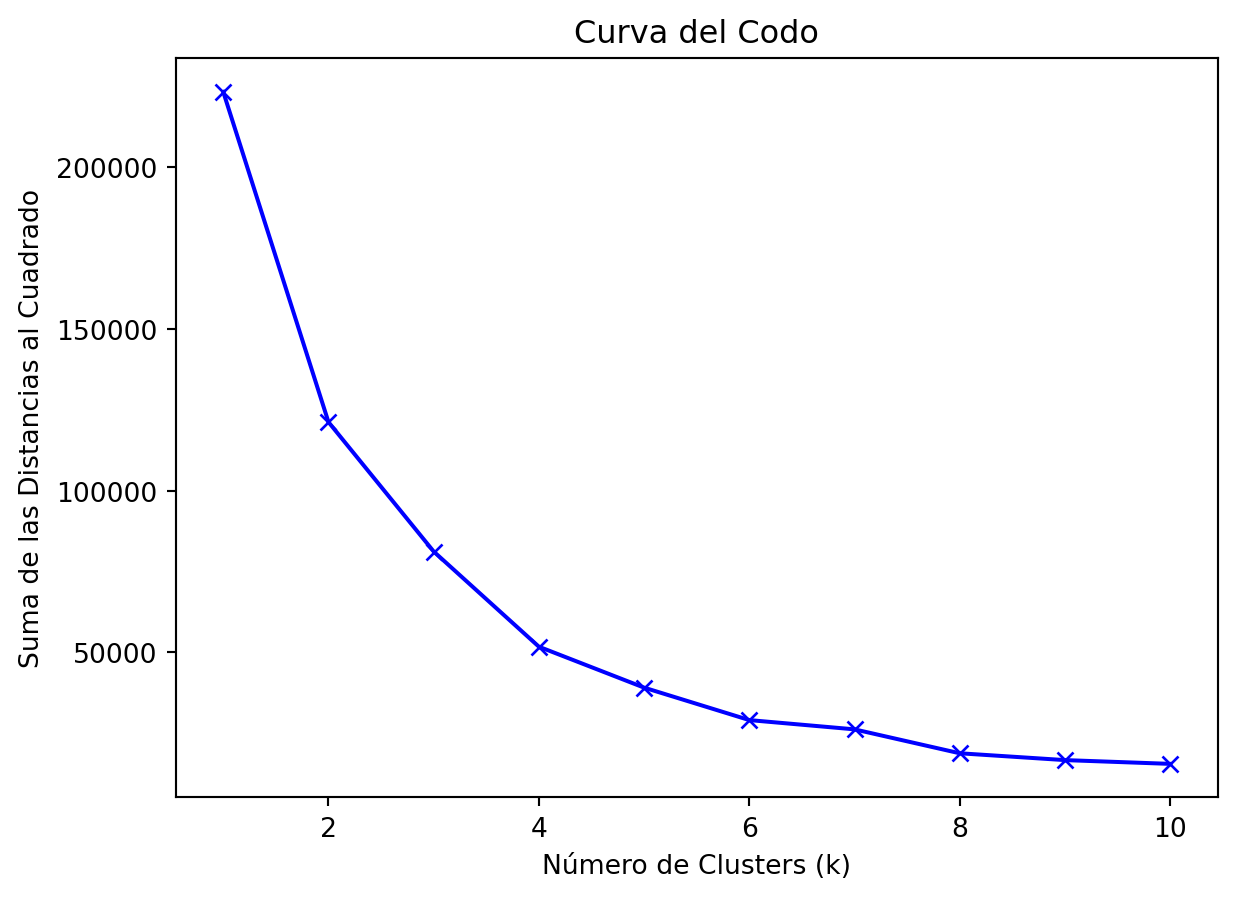
\includegraphics[scale=0.7]{imagenes/codo.png}
\caption{Curva del codo para determinar el número óptimo de clústers en el dataset de consumo eléctrico}
\end{figure}

Vemos que el valor de la inercia se estabiliza hasta $k=10$, lo que sugiere que
10 es el número óptimo de clústers para este conjunto de datos y no $k=8$ como se había supuesto inicialmente.
\cite{Rodríguez_Codo}